\documentclass[tikz,border=10pt]{standalone}
\usetikzlibrary{arrows.meta, positioning}

\begin{document}
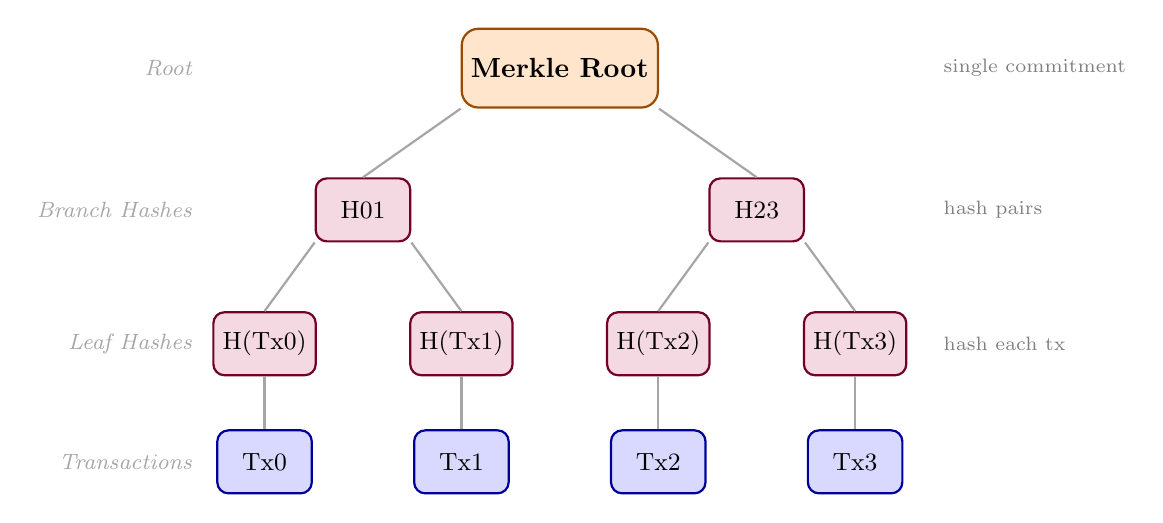
\begin{tikzpicture}[
  every node/.style={align=center},
  % Transaction nodes (leaves)
  tx/.style={rectangle, draw=blue!60!black, thick, rounded corners=4pt, fill=blue!15, minimum width=1.2cm, minimum height=0.8cm, font=\small},
  % Hash nodes (intermediate)
  hash/.style={rectangle, draw=purple!60!black, thick, rounded corners=4pt, fill=purple!15, minimum width=1.2cm, minimum height=0.8cm, font=\small},
  % Root node
  root/.style={rectangle, draw=orange!60!black, thick, rounded corners=6pt, fill=orange!20, minimum width=2cm, minimum height=1cm, font=\normalsize\bfseries},
  % Edges
  edge/.style={thick, draw=gray!70},
  % Labels
  label/.style={font=\footnotesize\itshape, text=gray!70}
]

% === LEVEL 0: Transactions ===
\node[tx] (tx0) at (0, 0) {Tx0};
\node[tx] (tx1) at (2.5, 0) {Tx1};
\node[tx] (tx2) at (5, 0) {Tx2};
\node[tx] (tx3) at (7.5, 0) {Tx3};

% Level label
\node[label, anchor=east] at (-0.8, 0) {Transactions};

% === LEVEL 1: Leaf Hashes ===
\node[hash] (h0) at (0, 1.5) {H(Tx0)};
\node[hash] (h1) at (2.5, 1.5) {H(Tx1)};
\node[hash] (h2) at (5, 1.5) {H(Tx2)};
\node[hash] (h3) at (7.5, 1.5) {H(Tx3)};

% Level label
\node[label, anchor=east] at (-0.8, 1.5) {Leaf Hashes};

% Edges: Tx -> Hash
\draw[edge] (tx0.north) -- (h0.south);
\draw[edge] (tx1.north) -- (h1.south);
\draw[edge] (tx2.north) -- (h2.south);
\draw[edge] (tx3.north) -- (h3.south);

% === LEVEL 2: Branch Hashes ===
\node[hash] (h01) at (1.25, 3.2) {H01};
\node[hash] (h23) at (6.25, 3.2) {H23};

% Level label
\node[label, anchor=east] at (-0.8, 3.2) {Branch Hashes};

% Edges: Leaf -> Branch
\draw[edge] (h0.north) -- (h01.south west);
\draw[edge] (h1.north) -- (h01.south east);
\draw[edge] (h2.north) -- (h23.south west);
\draw[edge] (h3.north) -- (h23.south east);

% === LEVEL 3: Merkle Root ===
\node[root] (root) at (3.75, 5) {Merkle Root};

% Level label
\node[label, anchor=east] at (-0.8, 5) {Root};

% Edges: Branch -> Root
\draw[edge] (h01.north) -- (root.south west);
\draw[edge] (h23.north) -- (root.south east);

% === Annotations ===
\node[font=\scriptsize, text=gray, anchor=west] at (8.5, 1.5) {hash each tx};
\node[font=\scriptsize, text=gray, anchor=west] at (8.5, 3.2) {hash pairs};
\node[font=\scriptsize, text=gray, anchor=west] at (8.5, 5) {single commitment};

\end{tikzpicture}
\end{document}
